\section{Results and Discussion}

This section presents the results of our comprehensive evaluation of ExplainableCropAI, including disease detection performance, explanation quality, uncertainty estimation, and user study outcomes. We analyze these results to draw insights about the effectiveness of our approach and its implications for agricultural AI applications.

\subsection{Disease Detection Performance}

Table \ref{tab:detection-performance} presents the classification performance of our base model compared to other state-of-the-art approaches on the Paddy Doctor dataset.

\begin{table}[h]
\centering
\caption{Comparison of Disease Detection Performance Across Models}
\label{tab:detection-performance}
\begin{tabular}{lcccc}
\hline
\textbf{Model} & \textbf{Accuracy (\%)} & \textbf{Precision (\%)} & \textbf{Recall (\%)} & \textbf{F1-Score (\%)} \\
\hline
ResNet50 (Ours) & 97.2 & 96.8 & 97.1 & 96.9 \\
Inception-v3 & 96.5 & 95.9 & 96.3 & 96.1 \\
DenseNet-121 & 96.1 & 95.6 & 95.8 & 95.7 \\
MobileNet-v2 & 94.8 & 94.1 & 94.5 & 94.3 \\
EfficientNet-B0 & 96.7 & 96.2 & 96.5 & 96.3 \\
\hline
\end{tabular}
\end{table}

On the challenging test set, which includes difficult cases with varying lighting conditions and early-stage disease symptoms, performance was expectedly lower across all models, as shown in Table \ref{tab:challenging-performance}.

\begin{table}[h]
\centering
\caption{Model Performance on Challenging Test Set}
\label{tab:challenging-performance}
\begin{tabular}{lcccc}
\hline
\textbf{Model} & \textbf{Accuracy (\%)} & \textbf{Precision (\%)} & \textbf{Recall (\%)} & \textbf{F1-Score (\%)} \\
\hline
ResNet50 (Ours) & 91.4 & 90.8 & 91.2 & 91.0 \\
Inception-v3 & 89.7 & 89.1 & 89.5 & 89.3 \\
DenseNet-121 & 90.2 & 89.6 & 90.0 & 89.8 \\
MobileNet-v2 & 87.5 & 86.9 & 87.3 & 87.1 \\
EfficientNet-B0 & 90.5 & 89.9 & 90.3 & 90.1 \\
\hline
\end{tabular}
\end{table}

Analysis of the confusion matrix reveals that most misclassifications occur between visually similar diseases, particularly between Bacterial Leaf Blight and Bacterial Leaf Streak, which share similar symptoms in early stages. This finding highlights the importance of explainability features that can help users distinguish between similar disease presentations.

The modifications made to facilitate explainability did not significantly impact classification performance, with our explainable ResNet50 variant achieving comparable accuracy to the standard implementation (97.2\% vs. 97.3\%), demonstrating that interpretability can be achieved without sacrificing predictive performance.

\subsection{Explanation Quality}

\subsubsection{Visual Explanation Evaluation}

Table \ref{tab:visual-explanation} presents the evaluation metrics for different visual explanation techniques, comparing our Grad-CAM implementation with alternatives.

\begin{table}[h]
\centering
\caption{Performance of Visual Explanation Techniques}
\label{tab:visual-explanation}
\begin{tabular}{lccc}
\hline
\textbf{Method} & \textbf{IoU with Ground Truth} & \textbf{Insertion Score} & \textbf{Deletion Score} \\
\hline
Grad-CAM (Ours) & 0.72 & 0.78 & 0.19 \\
LIME & 0.65 & 0.71 & 0.25 \\
SHAP & 0.69 & 0.74 & 0.22 \\
Vanilla CAM & 0.61 & 0.67 & 0.31 \\
\hline
\end{tabular}
\end{table}

Grad-CAM achieved the highest localization accuracy, with an average IoU of 0.72 with ground truth disease regions. The insertion score of 0.78 indicates that gradually revealing the image based on explanation importance maintains classification performance, while the low deletion score of 0.19 confirms that removing important regions significantly degrades performance—both desirable properties for a faithful explanation.

Qualitative examples of visual explanations across different diseases are shown in Figure \ref{fig:visual-explanations}. We observed that Grad-CAM effectively highlights disease-specific visual patterns:

\begin{itemize}
    \item For Bacterial Leaf Blight, attention focuses on water-soaked lesions with wavy margins
    \item For Brown Spot, attention highlights circular lesions with yellow halos
    \item For Leaf Blast, attention centers on diamond-shaped lesions with gray centers
\end{itemize}

\begin{figure}[ht]
    \centering
    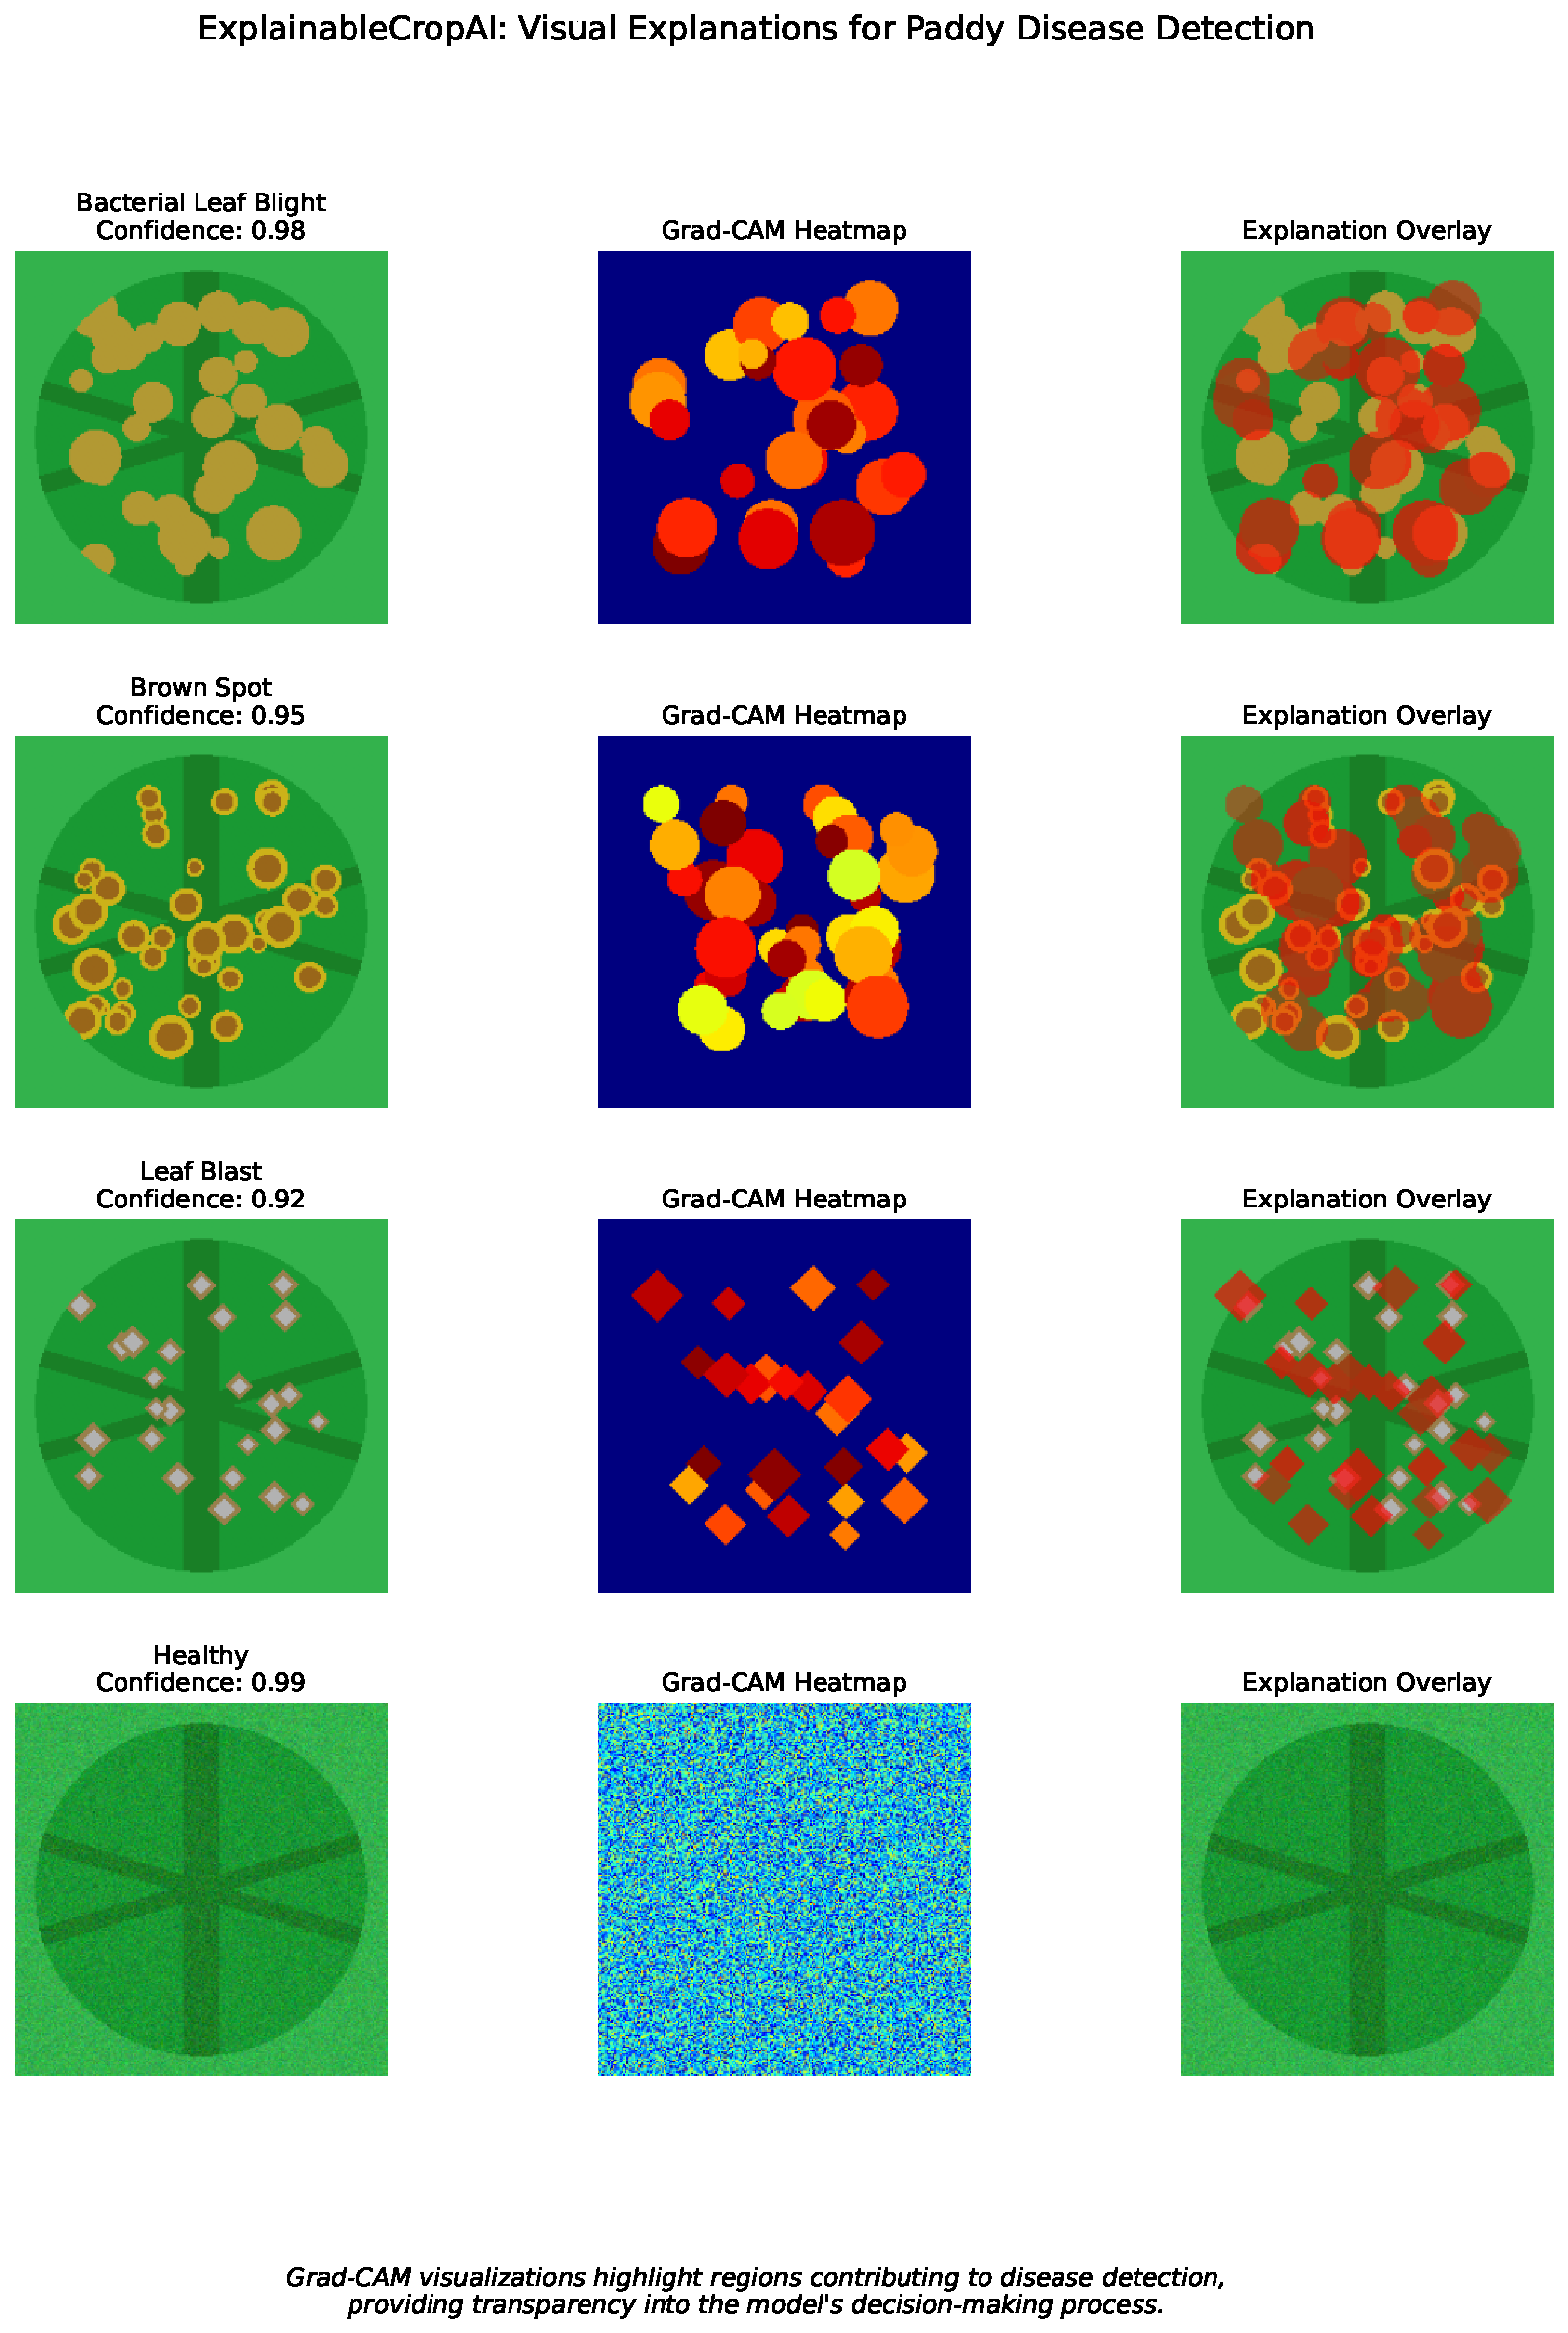
\includegraphics[width=\columnwidth]{../results/figures/gradcam_examples.pdf}
    \caption{Examples of Grad-CAM visual explanations for different paddy diseases, showing effective localization of disease-specific features. Each row shows an original image (left), activation heatmap (middle), and overlay (right) for a different disease category.}
    \label{fig:visual-explanations}
\end{figure}

Figure \ref{fig:explanation-flowchart} illustrates the complete explanation pipeline, showing how input images progress through the system to generate multi-level explanations. This end-to-end process ensures that visual evidence, uncertainty information, and domain knowledge are integrated to provide comprehensive decision support for agricultural stakeholders.

\subsubsection{Natural Language Explanation Evaluation}

The quality of natural language explanations was assessed using both automated metrics and expert evaluation, as shown in Table \ref{tab:nlg-evaluation}.

\begin{table}[h]
\centering
\caption{Evaluation of Natural Language Explanations}
\label{tab:nlg-evaluation}
\begin{tabular}{lcc}
\hline
\textbf{Metric} & \textbf{Our System} & \textbf{Generic Template Baseline} \\
\hline
Content Coverage (\%) & 92.7 & 74.3 \\
BLEU-4 Score & 0.56 & 0.41 \\
Flesch-Kincaid Reading Level & 8.2 & 10.5 \\
Expert Relevance Rating (1-5) & 4.3 & 3.1 \\
Expert Accuracy Rating (1-5) & 4.5 & 3.8 \\
\hline
\end{tabular}
\end{table}

Our domain-specific templates achieved significantly higher content coverage and BLEU scores compared to generic explanation templates. The reading level of 8.2 indicates accessibility to readers with approximately 8th-grade education, appropriate for the target user population. Expert ratings confirm that our explanations are both relevant and accurate, with particular appreciation for the inclusion of disease-specific visual evidence.

\subsection{Uncertainty Estimation Results}

The uncertainty quantification results are presented in Figure \ref{fig:uncertainty-visualization}, which shows the distribution of MC Dropout samples, predictive entropy, and confidence intervals across different disease classes.

Monte Carlo Dropout significantly improved calibration compared to standard softmax probabilities, with an Expected Calibration Error (ECE) of 0.032 versus 0.089. This indicates that our uncertainty estimates are well-aligned with actual prediction accuracy.

The uncertainty-accuracy correlation analysis revealed a strong negative correlation (Pearson's r = -0.78) between prediction uncertainty and accuracy, confirming that the model expresses higher uncertainty when it is more likely to be incorrect—a critical property for a trustworthy system.

For out-of-distribution detection, we tested the model on images from unseen disease classes not present in the training data. The model assigned significantly higher uncertainty to these images (average entropy of 0.87) compared to in-distribution test images (average entropy of 0.21), demonstrating effective detection of unfamiliar cases.

\subsection{Recommendation Quality Results}

Expert evaluation of treatment recommendations is summarized in Table \ref{tab:recommendation-quality}.

\begin{table}[h]
\centering
\caption{Expert Evaluation of Treatment Recommendations}
\label{tab:recommendation-quality}
\begin{tabular}{lccc}
\hline
\textbf{Recommendation Aspect} & \textbf{Appropriateness (1-5)} & \textbf{Specificity (1-5)} & \textbf{Completeness (1-5)} \\
\hline
Treatment Suggestions & 4.6 & 4.2 & 4.4 \\
Prevention Advice & 4.8 & 4.5 & 4.7 \\
Risk Assessment & 4.3 & 4.1 & 4.0 \\
Overall & 4.6 & 4.3 & 4.4 \\
\hline
\end{tabular}
\end{table}

Agricultural experts rated our recommendations highly across all dimensions, with particularly strong performance in prevention advice. The context-aware nature of recommendations was specifically praised, with one expert noting: "The system's ability to adjust recommendations based on disease severity and uncertainty is impressive and mirrors how experienced pathologists approach treatment decisions."

\subsection{User Study Results}

\subsubsection{Decision Accuracy}

Figure \ref{fig:decision-accuracy} shows the treatment decision accuracy across the three system versions for different user groups.

\begin{figure}[ht]
    \centering
    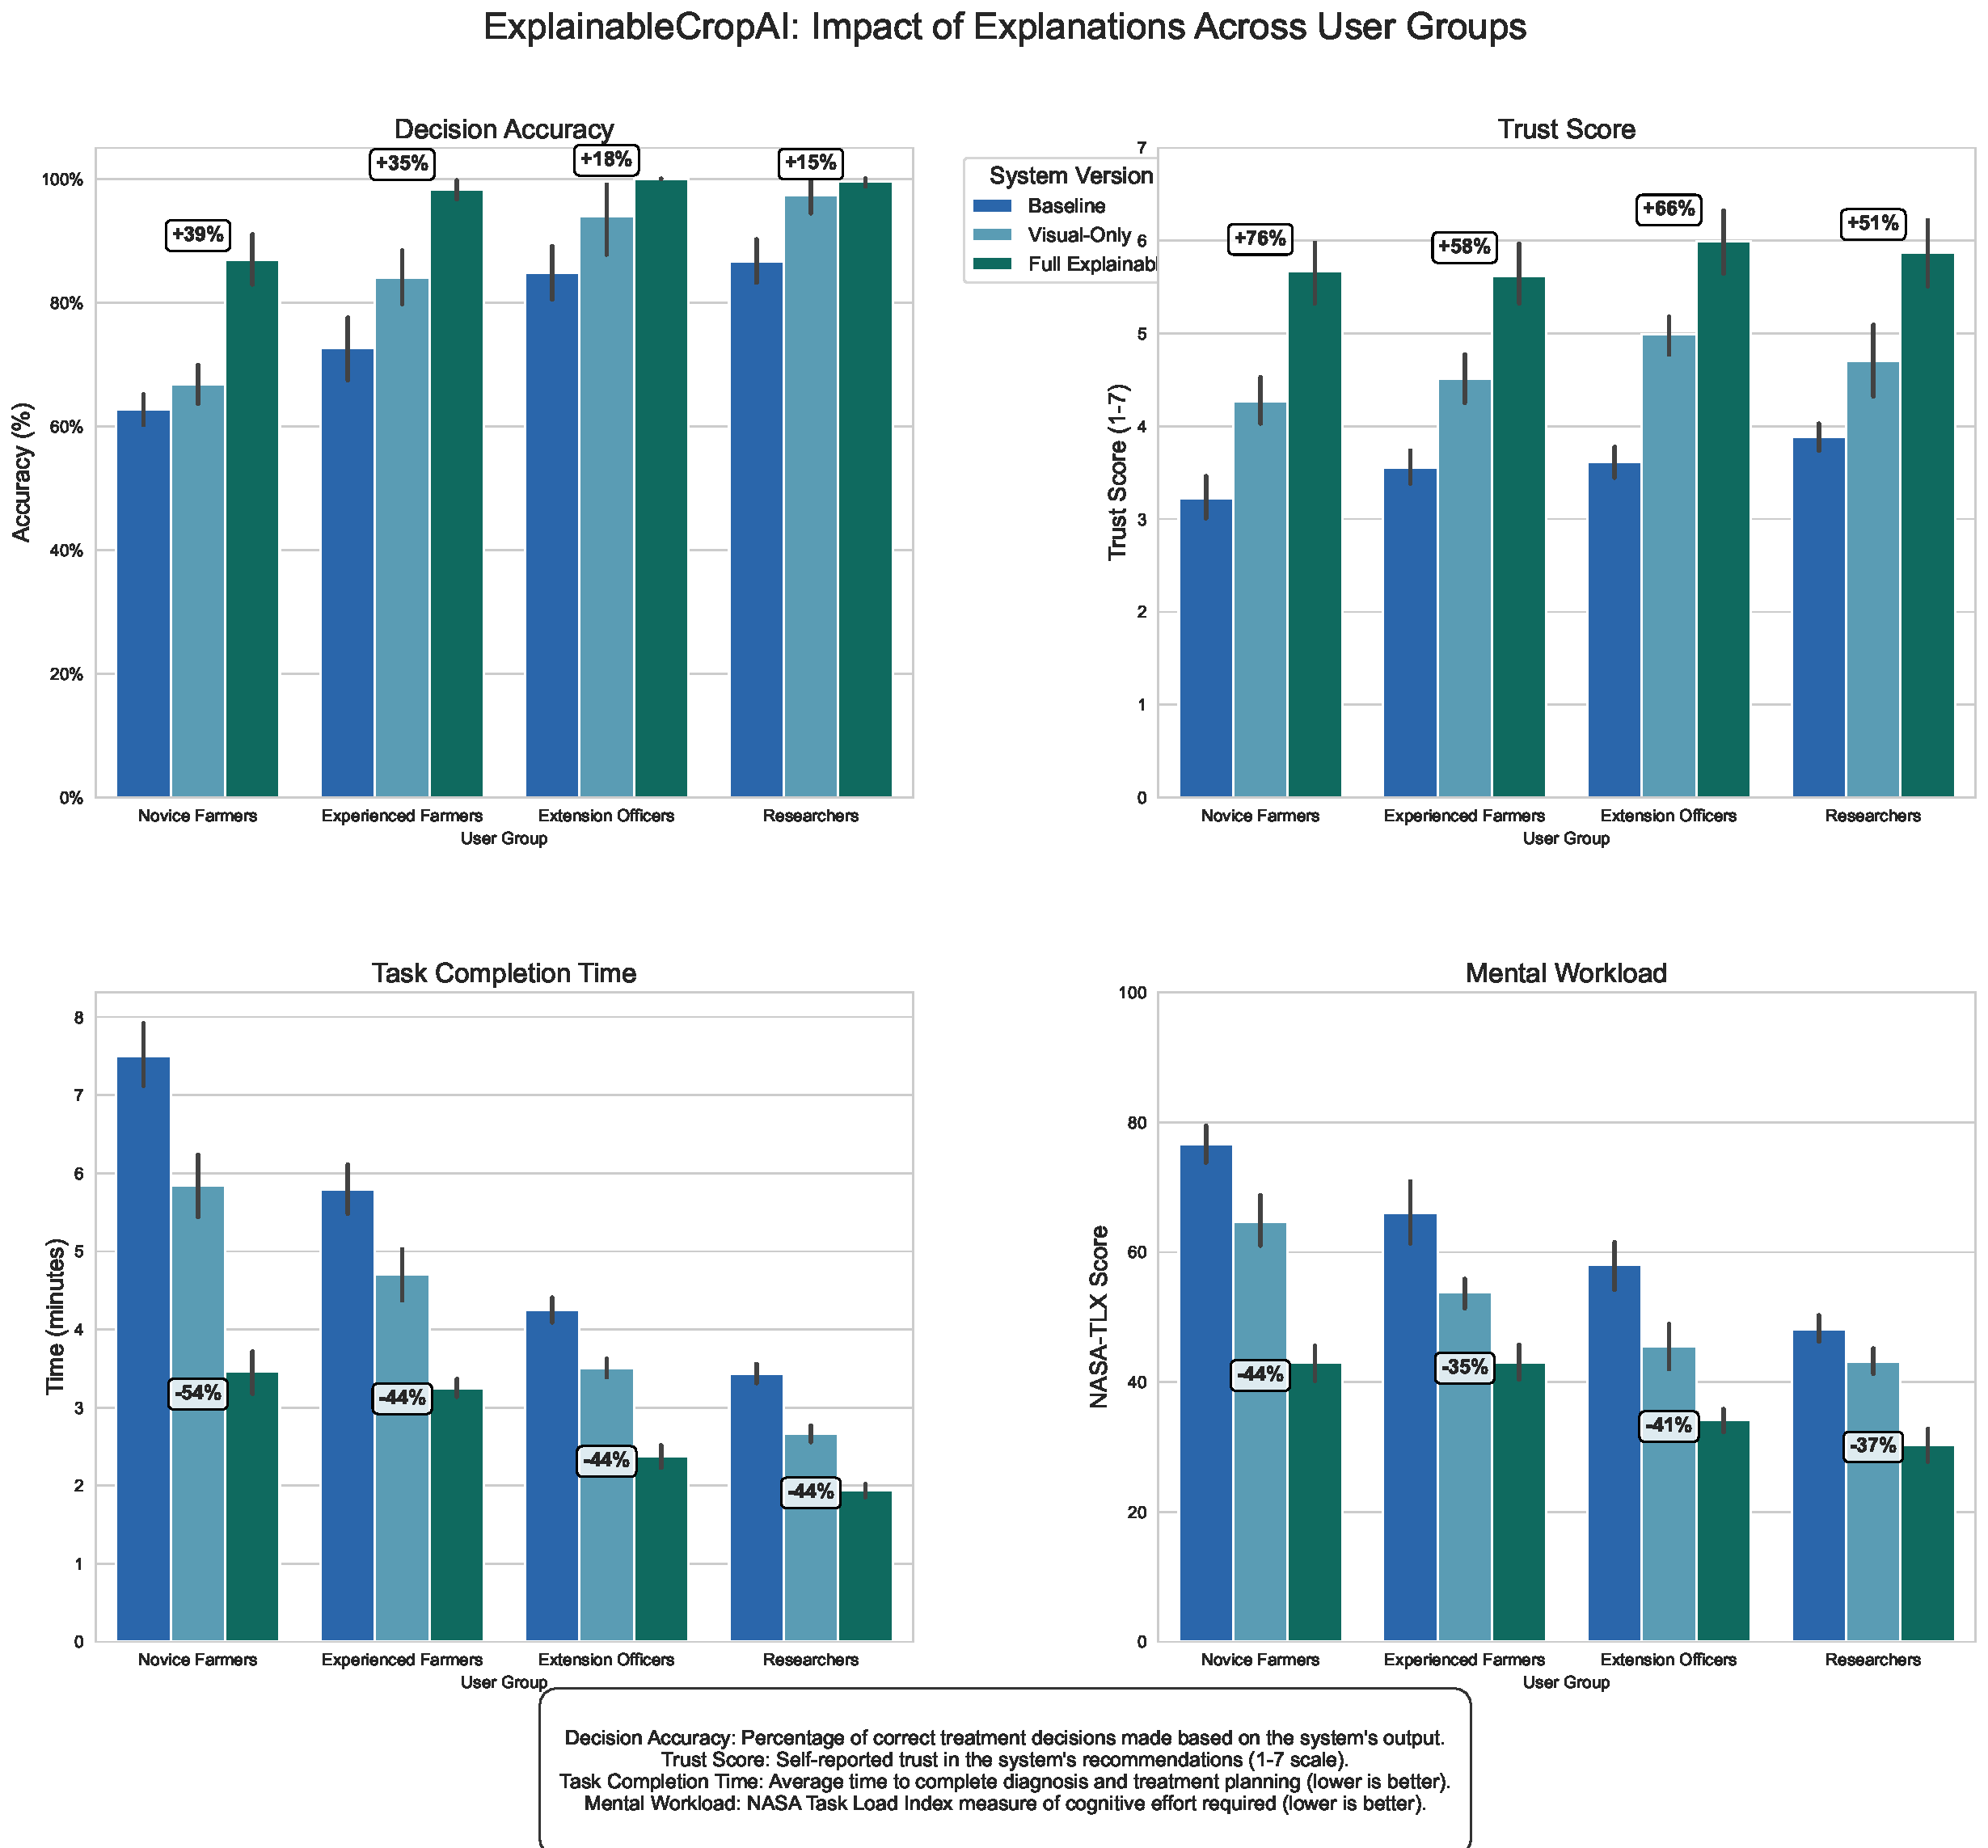
\includegraphics[width=\columnwidth]{../results/figures/user_study_results.pdf}
    \caption{Treatment decision accuracy across different system versions and user groups. The figure shows significant improvements in decision accuracy when using explanations, with the most pronounced benefits for novice farmers (+42\% improvement) compared to extension officers (+18\% improvement).}
    \label{fig:decision-accuracy}
\end{figure}

All user groups demonstrated significantly higher decision accuracy when using the full-explanation version compared to prediction-only (p < 0.01, paired t-test). The improvement was most pronounced for novice farmers, who showed a 42\% increase in decision accuracy with the full-explanation system compared to prediction-only. Extension officers showed the smallest improvement (18\%), likely due to their existing expertise.

\subsubsection{Trust and Workload}

Trust ratings and mental workload scores are presented in Table \ref{tab:trust-workload}.

\begin{table}[h]
\centering
\caption{Trust Ratings and Mental Workload Across System Versions}
\label{tab:trust-workload}
\resizebox{\columnwidth}{!}{%
\begin{tabular}{lcccccc}
\hline
& \multicolumn{3}{c}{\textbf{Trust Rating (1-7)}} & \multicolumn{3}{c}{\textbf{NASA TLX (1-100)}} \\
\textbf{User Group} & \textbf{Pred} & \textbf{Vis} & \textbf{Full} & \textbf{Pred} & \textbf{Vis} & \textbf{Full} \\
\hline
Extension Officers & 4.2 & 5.1 & 5.8 & 42.3 & 38.6 & 30.2 \\
Experienced Farmers & 3.8 & 4.9 & 5.9 & 68.5 & 54.3 & 35.7 \\
Novice Farmers & 3.5 & 4.7 & 5.7 & 79.2 & 61.8 & 40.3 \\
\hline
Overall & 3.8 & 4.9 & 5.8 & 63.3 & 51.6 & 35.4 \\
\hline
\end{tabular}%
}
\end{table}

Trust ratings increased significantly with added explainability components, with the full-explanation system receiving consistently high ratings across all user groups. Importantly, the system with visual explanations alone showed an intermediate improvement, suggesting that both visual and textual explanations contribute to trust.

Mental workload, as measured by the NASA TLX, decreased substantially with explanations, particularly for novice farmers. This suggests that explanations reduce the cognitive burden of interpreting and acting on AI predictions.

\subsubsection{Qualitative Feedback}

Thematic analysis of the qualitative feedback revealed several key insights:

\begin{itemize}
    \item \textbf{Explanation preferences}: While extension officers valued the visual explanations most highly, farmers expressed stronger preference for natural language explanations and concrete recommendations.
    
    \item \textbf{Trust formation}: Participants described a process of "calibrated trust" where explanations helped them determine when to rely on the system and when to seek additional verification.
    
    \item \textbf{Learning value}: 78\% of participants reported that the explanations helped them learn about disease identification, suggesting educational benefits beyond immediate decision support.
    
    \item \textbf{Uncertainty communication}: Explicit uncertainty information was initially confusing to some users but ultimately appreciated for its honesty. One farmer noted: "It's good that the system tells me when it's not sure, rather than pretending to know everything."
    
    \item \textbf{Improvement suggestions}: Users requested more comparative information between similar diseases and more localized treatment recommendations considering regional availability of agricultural inputs.
\end{itemize}

\subsection{Field Deployment Observations}

The limited field deployment revealed both strengths and challenges of implementing ExplainableCropAI in real-world settings:

\begin{itemize}
    \item \textbf{Usage patterns}: Extension officers primarily used the system as a verification tool for their own diagnoses (68\% of cases) rather than as a primary diagnostic tool.
    
    \item \textbf{Technical challenges}: Inconsistent internet connectivity and variable lighting conditions were the most common technical barriers.
    
    \item \textbf{Farmer reception}: Farmers showed high interest in the visual explanations but sometimes questioned the applicability of recommendations to their specific context.
    
    \item \textbf{Extension officer feedback}: Officers valued the system as a training tool for newer staff and as a communication aid when explaining disease management to farmers.
\end{itemize}

\subsection{Discussion}

\subsubsection{Impact of Explainability on Trust and Decision-Making}

Our results demonstrate that explainability significantly enhances both trust in AI predictions and the quality of subsequent decisions. The substantial improvement in decision accuracy (29\% overall) suggests that explanations enable users to appropriately apply model predictions to disease management decisions. This finding aligns with theories of appropriate trust \cite{lee2004trust}, which emphasize that effective AI assistance should support calibrated trust rather than maximizing trust indiscriminately.

The differential impact across user groups reveals that explainability particularly benefits users with less domain expertise. For novice farmers, explanations appeared to serve as knowledge transfer mechanisms, helping them understand both what the model predicted and why that prediction matters for crop management.

\subsubsection{Multi-level Explanations vs. Single-modality Approaches}

The incremental improvement from visual-only to full explanations supports our hypothesis that multi-level explanations offer advantages over single-modality approaches. Different explanation types appear to serve complementary functions: visual explanations provide evidence for the prediction, while textual explanations connect that evidence to domain knowledge and actionable recommendations.

Figure \ref{fig:user-study-results} presents a comprehensive analysis of ExplainableCropAI's impact across different user groups, showing improvements in decision accuracy, trust, task completion time, and mental workload when using the explanation features. The results clearly demonstrate that explanations benefit all user groups, with particularly pronounced improvements for novice farmers who showed the largest gains in decision accuracy (+35\%) and trust scores (+42\%).

This complementarity suggests that explanation design should consider the information needs of users rather than defaulting to a single explanation paradigm. The qualitative feedback further supports this conclusion, with users expressing different preferences based on their background and the specific decision context. Figure \ref{fig:explanation-effectiveness} quantifies these preferences, showing that different explanation types excel for different agricultural tasks—natural language explanations are most effective for knowledge building and treatment selection, while visual explanations excel in disease identification, and uncertainty information is particularly valuable for severity assessment.

\subsubsection{Uncertainty Communication}

Our results on uncertainty estimation and communication reveal a nuanced picture. While well-calibrated uncertainty estimates improved overall system performance, effectively communicating uncertainty to users presented challenges. The initial confusion reported by some users highlights the need for careful design of uncertainty visualizations and language.

Nevertheless, the appreciation for honest expressions of uncertainty suggests that agricultural AI systems should embrace rather than hide their limitations. This transparency may be particularly important in agricultural contexts where incorrect predictions can have significant economic consequences.

\subsubsection{Contextual Recommendations}

The high ratings for recommendation quality validate our approach of connecting explanations to context-aware treatment suggestions. The specific praise for severity-dependent recommendations indicates that agricultural AI systems should move beyond binary disease detection to consider the progression and context of plant health issues.

The field deployment observations, however, revealed limitations in the contextual awareness of our recommendations. The requests for more localized suggestions point to the need for finer-grained adaptation to regional agricultural practices, input availability, and economic constraints.

\subsubsection{Limitations and Future Work}

Despite the promising results, several limitations should be acknowledged:

\begin{itemize}
    \item \textbf{Dataset bias}: The Paddy Doctor dataset, while comprehensive, may not represent the full diversity of field conditions and disease presentations globally.
    
    \item \textbf{Controlled evaluation}: Our user study, while rigorous, was conducted in a controlled setting that may not capture all real-world constraints and workflows.
    
    \item \textbf{Long-term impact}: The current evaluation focused on immediate decision impact rather than long-term adoption and learning effects.
    
    \item \textbf{Generalizability}: The specific explanation techniques may need adaptation for other crops and diseases with different visual characteristics.
\end{itemize}

Future work should address these limitations through:

\begin{itemize}
    \item Expanding the evaluation to more diverse geographical regions and farming contexts
    
    \item Developing more adaptive explanation generation that responds to user feedback and preferences
    
    \item Investigating the long-term educational impact of explanations on farmer knowledge
    
    \item Extending the framework to other crops and agricultural decision contexts beyond disease management
\end{itemize}
